% Systematisk beskrivelse af konfigurations tabel.
\section{Konfigurationstabel}\label{konfigurationstabel}
En konfiguration af et system er en kombination af sammenhængende elementer, og en konfigurationstabel beskriver den konfiguration.
For et projekt vil der være en lang række konfigurationer, hvor imellem enhver konfiguration vil der være ændringer i én eller flere celler i konfigurationstabellen.
Konfigurationstabellen holdes opdateret løbende for at holde et fælles og enigt overblik over projektet.
I \cref{tab:konfigurationsTabel} præsenteres den endelige konfigurationstabel for projektet, og indholdet vil i de følgende afsnit blive nærmere forklaret.

\begin{figure}
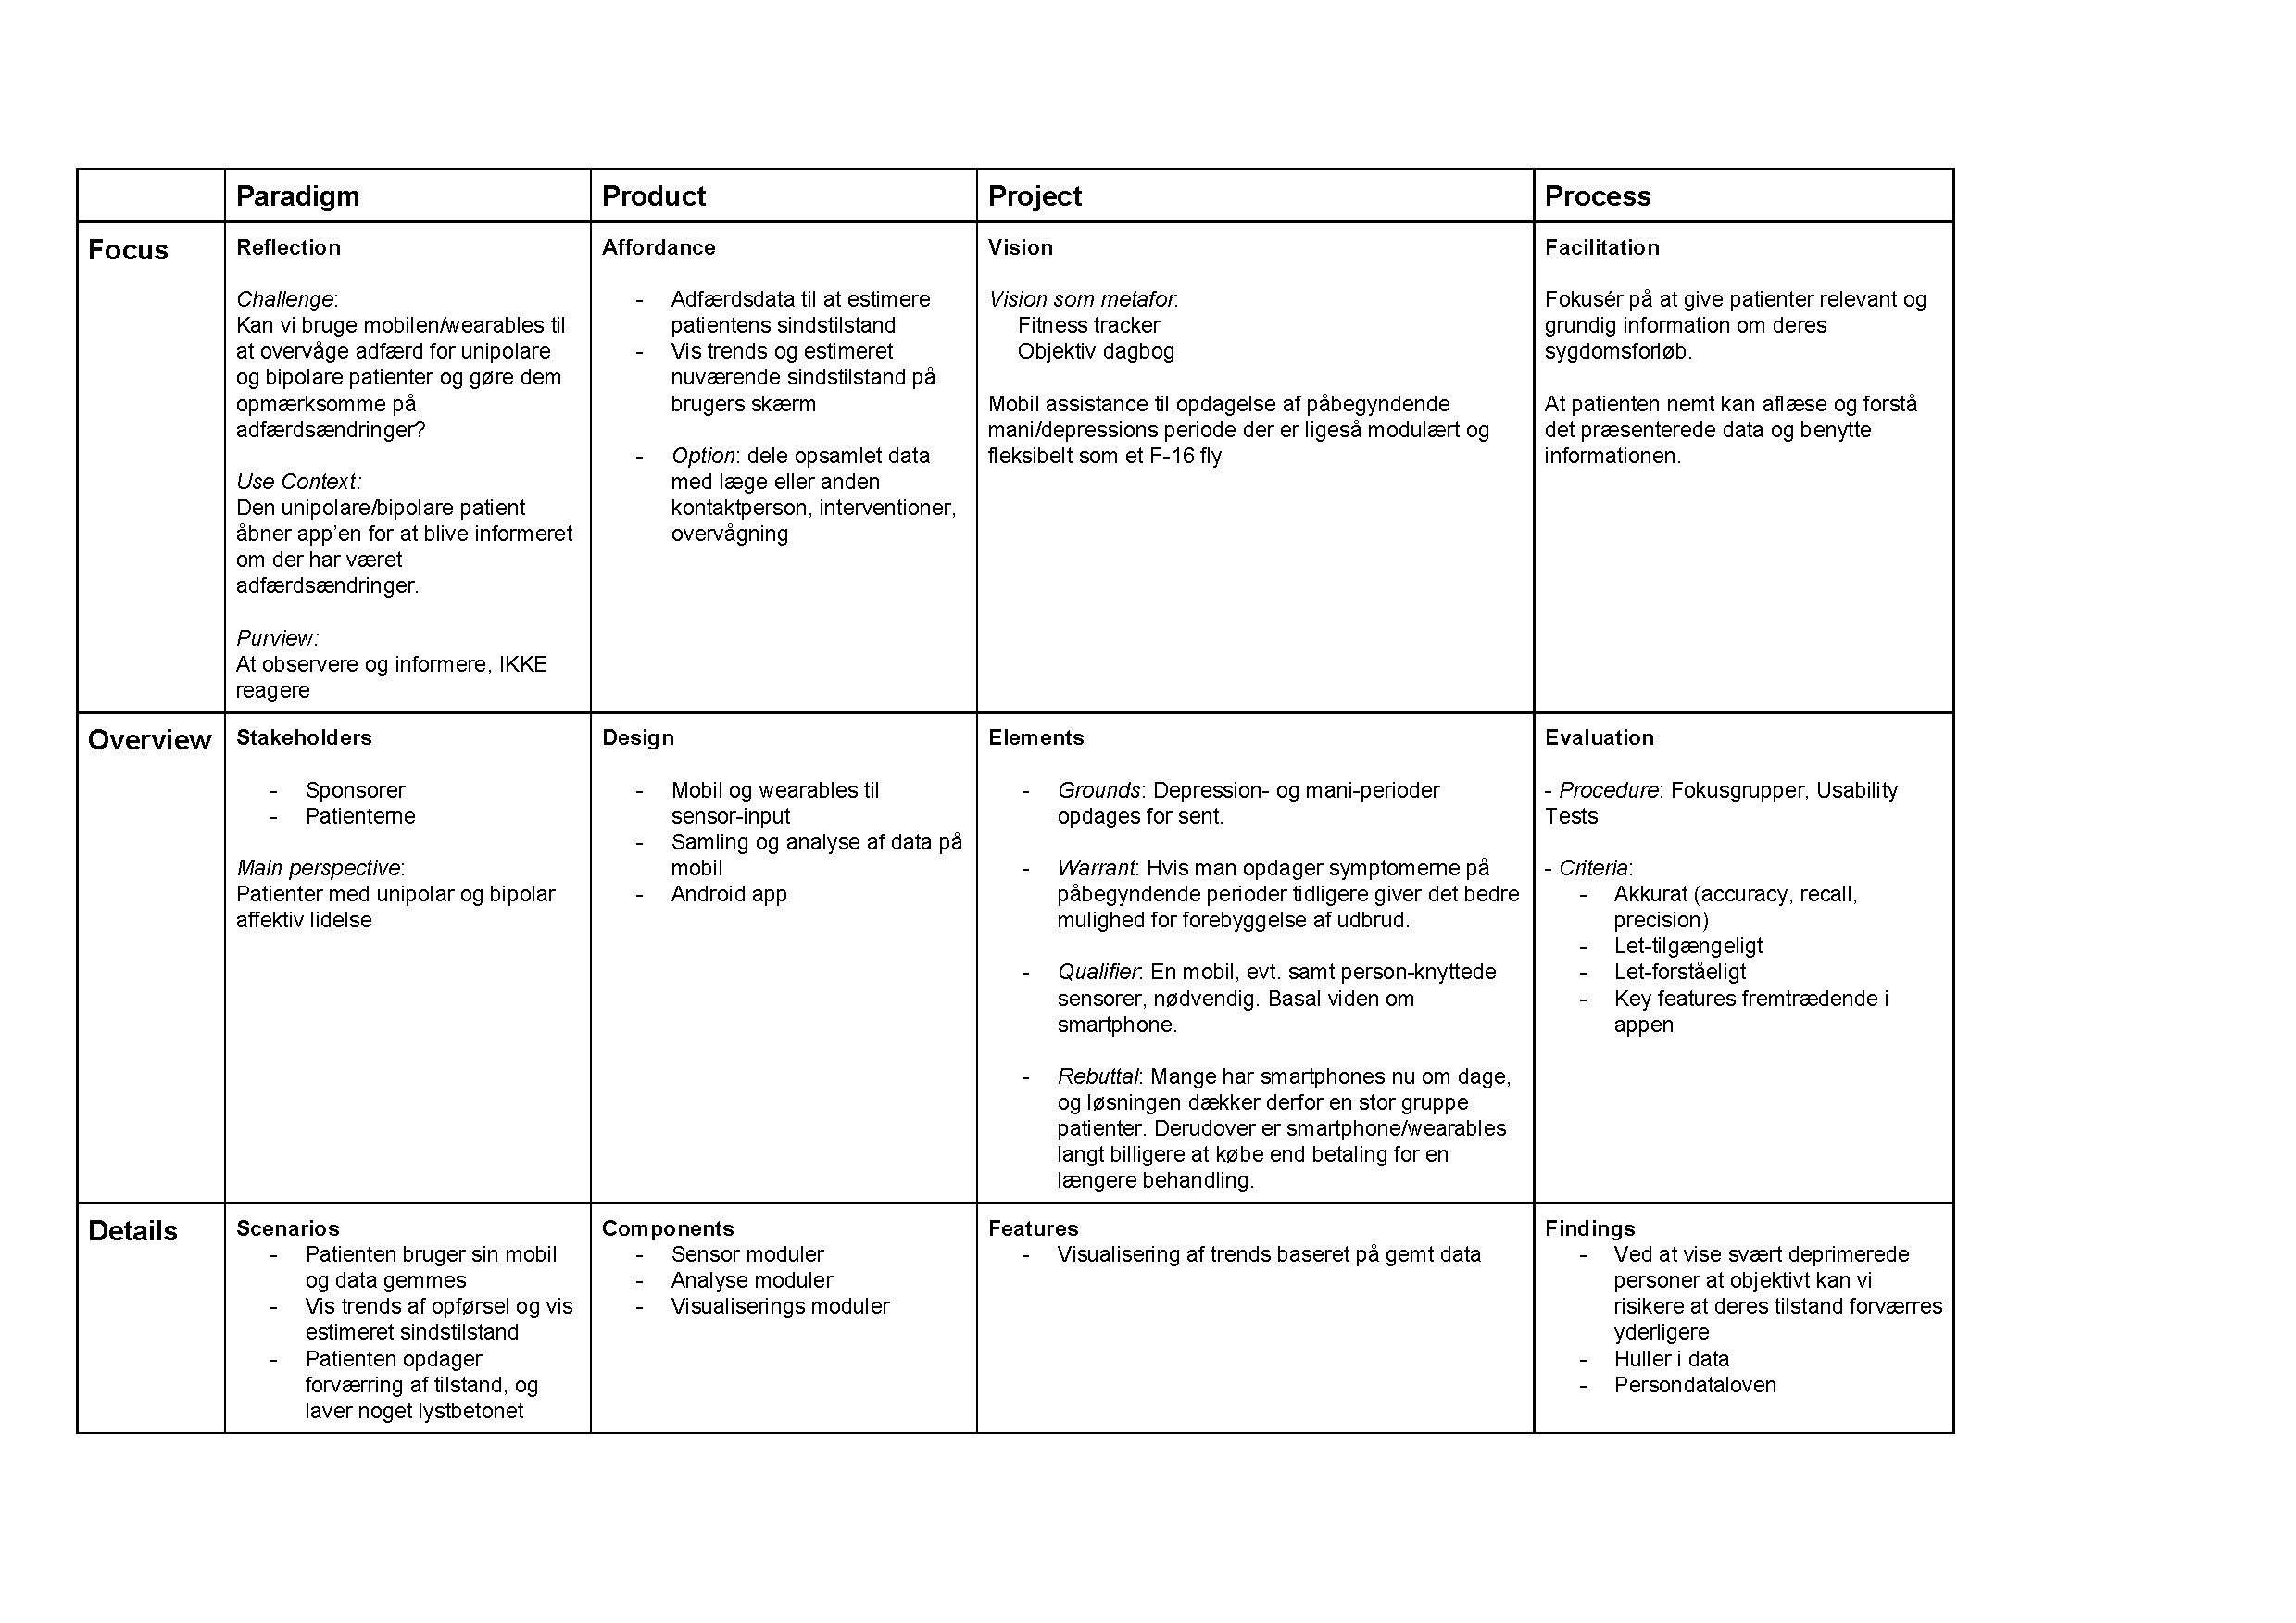
\includegraphics[scale = 0.65,trim = 1cm 3cm 6cm 2cm, angle = 90, clip]{KonfigurationTabel}
\caption{Konfigurations tabellen for systemet.}
\label{tab:konfigurationsTabel}
\end{figure}
